\documentclass[10pt]{article}
\usepackage{a4wide}
\usepackage[english]{babel}
\usepackage{graphicx}
\usepackage{tabu}
\usepackage{textcomp}
\usepackage{fancyhdr}
\usepackage{lastpage}
\usepackage{titlesec}
\usepackage{pdflscape}
\usepackage{longtable}
\usepackage{color}
\usepackage{listings}
\usepackage{xkeyval}
\usepackage{hyperref}
\usepackage{wrapfig}
\usepackage{rotating}
\usepackage{epstopdf}

\definecolor{mygreen}{rgb}{0,0.6,0}
\definecolor{mygray}{rgb}{0.5,0.5,0.5}
\definecolor{mymauve}{rgb}{0.58,0,0.82}

\lstset{ % Syntax highliughting for java
  backgroundcolor=\color{white},   % choose the background color; you must add \usepackage{color} or \usepackage{xcolor}
  basicstyle=\footnotesize,        % the size of the fonts that are used for the code
  breakatwhitespace=false,         % sets if automatic breaks should only happen at whitespace
  breaklines=true,                 % sets automatic line breaking
  captionpos=b,                    % sets the caption-position to bottom
  commentstyle=\color{mygreen},    % comment style
  deletekeywords={...},            % if you want to delete keywords from the given language
  escapeinside={\%*}{*)},          % if you want to add LaTeX within your code
  extendedchars=true,              % lets you use non-ASCII characters; for 8-bits encodings only, does not work with UTF-8
  frame=none,                    % adds a frame around the code
  keepspaces=true,                 % keeps spaces in text, useful for keeping indentation of code (possibly needs columns=flexible)
  keywordstyle=\color{blue},       % keyword style
  language=Octave,                 % the language of the code
  morekeywords={*,...},            % if you want to add more keywords to the set
  numbers=left,                    % where to put the line-numbers; possible values are (none, left, right)
  numbersep=5pt,                   % how far the line-numbers are from the code
  numberstyle=\tiny\color{mygray}, % the style that is used for the line-numbers
  rulecolor=\color{black},         % if not set, the frame-color may be changed on line-breaks within not-black text (e.g. comments (green here))
  showspaces=false,                % show spaces everywhere adding particular underscores; it overrides 'showstringspaces'
  showstringspaces=false,          % underline spaces within strings only
  showtabs=false,                  % show tabs within strings adding particular underscores
  stepnumber=5,                    % the step between two line-numbers. If it's 1, each line will be numbered
  stringstyle=\color{mymauve},     % string literal style
  tabsize=4,                       % sets default tabsize to 2 spaces
  title=\lstname                   % show the filename of files included with \lstinputlisting; also try caption instead of title
}
%%%%%%
%% Variables for version and release status
%% useage: \version
%%%%%%
\newcommand\module{SE31520}
\newcommand\assignmentTitle{Weblog Assignment 1}
\newcommand\authorText{Nicholas Dart}
\newcommand\authorUsername{nid21}
\newcommand\studentID{130057750}
\newcommand\assesser{Some prof}

%%%%%%
%% Alias
%%%%%%
%\newcommand{\sectionbreak}{\clearpage}    %% Allways start a section on a new page

\title{ \huge \module~Assignment \\ \Large \assignmentTitle}
\author{
  \vspace{100pt}
  \begin{tabular}{ r || l }
    Author          & \authorText (\authorUsername)\\
            & \studentID \\
    Date Published  & \today \\
            & \\
    Assessed By     & \assesser \\
    Department      & Computer Science \\
    Address         & Aberystwyth University \\
            & Penglais Campas \\
            & Ceredigion \\
            & SY23 3DB \\
  \end{tabular} \\
  Copyright \textcopyright~Aberystwyth University 2015
  %get rid of the date on the titlepage
  \date{}
}

\pagestyle{fancy}
\fancyhf{}
\lhead{\module~Assignment}
\rhead{\authorText~-~\studentID}
\rfoot{Page \thepage \hspace{1pt} of \pageref{LastPage}}
\lfoot{Aberystwyth University - Computer Science}

\begin{document}
  % \setcounter{page}{1}

  % \maketitle
  % \thispagestyle{empty}
  % \clearpage

  % \tableofcontents
  % \clearpage

  Ruby on Rails applications follow the MVC Model\-View\-Controller design pattern, specifically the Model 2 variant. Model 2 differs from classical MVC by allowing a controller render a view without requiring a model. This is made use of in the Weblog application with the homepage/welcome page where a model is not desired to display the static text. \\

  The Weblog application consists of two models; a User (located in the file \textbf{app/models/user.rb}) and a Post (\textbf{app/model/post.rb}). The User model contains information about users in the system, including the user's first and last name and their email address. They are also assigned a unique ID. The post model contains a title and body of a post, and contains a foreign key to a user, by referring to their ID. A post also contains a unique ID. \\

  Views in the app are all based on a common template, within which subsequent views are rendered. This template (located in \textbf{app/views/layouts/application.erb.html}) contains the base HTML structure of all views to be rendered, and in the Weblog application, contains links to the Bootstrap stylesheet and Javascript resources, as well as adding page tabbing to the different views and wrapping all view contents in a Bootstrap container.

  The welcome page view (located in the file \textbf{app/views/welcome.erb.html}) contains an ``embedded ruby'' template that contains the HTML for the index page. ``Embedded ruby'' files contain HTML with some ruby to be executed that optionally can have their results embedded within the HTML after interpretation.

  The Users view contains multiple parts as CRUD behaviour is required. Several pages and partial pages are present (in \textbf{app/views/users/ directory}); a new User page, a list page for viewing all users and an individual user page and an edit page. The new, edit pages both use a partial page that contains a form as these elements are common to both pages. This layout is similarly structured in \textbf{app/views/posts/} directory. \\

  Views are rendered via Controllers, which can optionally provide a model with which to render the information. The controllers are responsible for routing CRUD requests to the relevant view components or responding with JSON if requested. In the Weblog application, the Users controller (located in the file \textbf{app/controllers/users\_controller.rb}) and the Posts controller (located in the file \textbf{app/controllers/posts\_controller.rb}) respond to incoming requests by retrieving any requested model and providing it to the relevant view component.


  \begin{landscape}
    % \section{Architecture Diagram}
      \begin{figure}
        \centering
          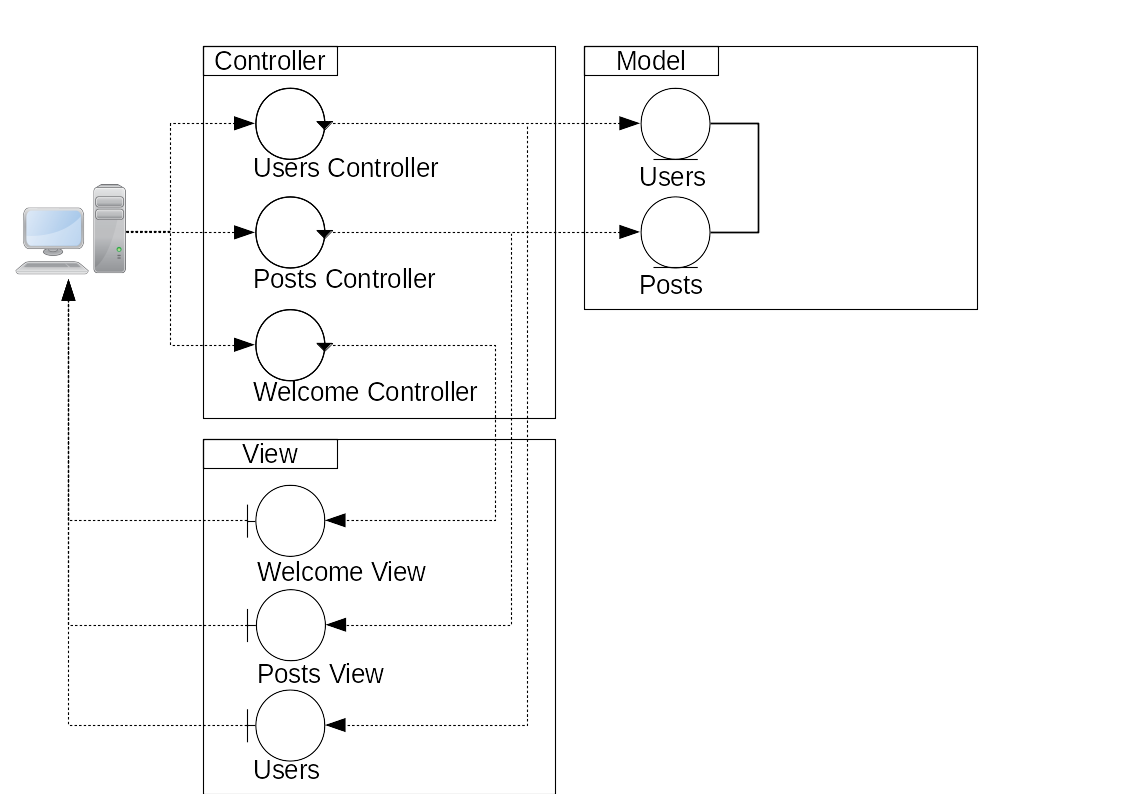
\includegraphics[height=\textheight]{uml.png}
        \caption{UML Diagram for the Weblog Project}
        \label{fig:gull}
      \end{figure}
    % Figure \ref{fig:gull} shows a photograph of a gull.
  \end{landscape}

\end{document}
